\documentclass[../Report.tex]{subfiles}
\usepackage[italian]{babel}
\graphicspath{ {../../Images/} }

\begin{document}
    \chapter{Valutazione del Design}
    In questo capitolo andremo a valutare quello che è il design ottenuto dalle fasi precedenti. La valutazione sarà formata da due step:
    \begin{itemize}
        \item \textbf{L'ispezione:} nella quale andremo a valutare noi stessi in qualità di membri del team il design ottenuto. Useremo la tecnica del \emph{cognitive walkthrougth}, una tecnica che sfrutta l'approccio drammaturgico narrativo, e l'\emph{analisi euristica} con le euristiche definite precedentemente.
        \item  \textbf{Il testing:} nella quale verra chiesto ad alcuni utenti di utilizzare i nostri wireframe per valutare l'usabilità del sito. 
    \end{itemize}

    \section{Ispezione}
    Per quanto riguarda l'ispezione stileremo dapprima una lista di task che vogliamo analizzare.
    \begin{enumerate}
        % SIMONE I PRIMI TRE - LUCA GLI ULTIMI 3
        \item Accedere al profilo
        \item Giocare al gioco "Subway surf", metterlo nei preferiti e lasciare un commento. Eliminare poi il commento.
        \item Cercare un utente e aggiungerlo alla lista degli amici.
        \item Modificare la propria foto profilo, caricandone una personalizzata.
        \item Eliminare un gioco dai preferiti.
        \item Impostare il parental control con un limite di due ore di utilizzo ed un blocco per i giochi che superino i 16 anni.
        \item Aggiungere al parental control il blocco per i giochi violenti.
        \item Disabilitare il parental control.
        \item Creare un nuovo account.
    \end{enumerate}
    \subsection{Cognitive Walkthrought}
    \subsubsection{Cognitive walkthrough 1:}
    \textbf{Task:} Accedere al profilo\\
    \textbf{User:} Una donna di 40 anni come Simona
    \subsubsection{Happy path}
    \begin{enumerate}
        \item Cliccare sull'icona dell'utente in alto a destra
        \item Cliccare su accedi con Facebook o Gogle qualora si volesse effettuare l'accesso tramite social network oppure inserire username e password negli appositi campi
        \item Cliccare su 'Accedi'
    \end{enumerate}
    \textbf{Walkthrough}:\\
    Simona si trova nell'Homepage del sito, individua il pulsante in alto con l'icona del profilo, la clicca e viene reindirizzata alla pagina di login.
    Inserisce l'username e la password ed in seguito ad un errore di battitura non digita la password corretta ed è costretto a modificare la password appena inserita e ripremere il pulsante 'Accedi'.

    \textbf{Valutazione:}\\Storia credibile e segue perfettamente l'happy path, è necessario che compaia un messaggio di errore in caso la password sia errata per un errore di battitura.\\

    \textbf{Miglioramenti:}Inserire un messaggio di errore in caso la password sia errata.\\

    \subsubsection{Cognitive walkthrough 2:}
    \textbf{Task:} Giocare al gioco "Subway surf", metterlo nei preferiti e lasciare un commento. Eliminare poi il commento.\\
    \textbf{User:} Un bambino dell'età di 12 anni come Mirko
    \subsubsection{Happy Path}
\begin{enumerate}
    \item Cliccare sull'icona di ricerca in alto a destra
    \item Digitare nel campo apposito 'Subway Surf'
    \item Cliccare su 'Invio'
    \item Cliccare sull'immagine riferita al gioco
    \item Cliccare il tastino del cuore ed eseguire l'accesso in caso non sia stato fatto
    \item Scorrere in fondo alla pagina
    \item Digitare il commento nella sezione apposta
    \item Cliccare sul pulsante con l'icona 'Invio'
    \item Cliccare poi sul menu (i tre puntini)
    \item Cliccare su Elimina 
\end{enumerate}
\textbf{Walkthrough}:\\
    Mirko si trova nell'homepage la scorre cercando il gioco di suo interesse e non lo trova.
    Di conseguenza clicca sul pulsante di ricerca e inizia a digitare 'Subway surf' fino che non compare come risultato.
    Una volta trovato lo clicca e viene reindirizzato alla pagina di suo interesse.
    Gioca per un paio di minuti al gioco e si accorge che questo gioco fa proprio al caso suo! Decide allora di volerlo mettere nella lista dei preferiti e clicca sul cuore in alto a destra. Vuole poi lasciare un commento scrivendo l'enorme punteggio che è riuscito a realizzare, clicca allora sul pulsante dei commenti sotto al cuore che lo reindirizza alla sezione dei commenti in fondo alla pagina.
    Nel campo di testo, digita un commento e successivamente preme invio per pubblicarlo. Si accorge di aver scritto un commento grammaticalmente sbagliato e decide di eliminarlo. Preme sul suo commento senza successo, ma nota poi alla destra il menu, ci clicca e clicca poi su elimina. Infine scrive il nuovo commento corretto. 

    \textbf{Valutazione:}\\Storia  realistica e abbastanza semplice.\\

    \textbf{Miglioramenti:}\\Nessuno.

    \subsubsection{Cognitive walkthrough 3:}
    \textbf{Task:} Cercare un utente e aggiungerlo alla lista degli amici.\\
    \textbf{User:} Un bambino dell'età di 8 anni come Gaetano
    \subsubsection{Happy Path}
    \begin{enumerate}
        \item Eseguire l'accesso qualora non sia stato fatto 
        \item Cliccare sull'immagine del profilo in alto a destra
        \item Selezionare nel menu a tendina la voce 'Amici'
        \item Qualora non fosse già selezionato, selezionare la tab 'I miei amici'
        \item Cliccare il pulsante con l'icona dell'utente e un '+'
        \item Digitare il nome dell'amico nel campo
        \item Mandargli la richiesta di amicizia con il tasto '+'
    \end{enumerate}
    \textbf{Walkthrough}:\\
    Gaetano vuole aggiungere agli amici il suo compagno di banco Lucio. Una volta eseguito l'accesso va nel menu a tendina riferita all'immagine del profilo dell'utente.
    Seleziona la voce 'Amici' e clicca sul pulsante 'Ricerca' digita il nome dell'utente ma non lo trova chiude quindi quella finestra e clicca sull'icona affianco con l'omino e il '+' si apre quindi un'altra barra di ricerca.
    Digita il nome dell'amico, lo trova e lo aggiunge alla lista degli amici.\\

    \textbf{Valutazione:}\\Storia non troppo realista poiché il ragazzo ha solo 8 anni e non è detto che sappia muoversi cosi bene su un sito se non con l'ausilio di un adulto.
    Nonostante il path è errato poiché per prima cosa l'utente cerca nella sua lista di amici e non trova il risultato sperato quindi è costretto a tornare indietro e trovare il pulsante 'aggiungi amici'.\\

    \textbf{Miglioramenti:} Mettere in risalto il fatto che la prima ricerca si basa solo sugli amici gia nella lista e non dei nuovi. Aggiungeremo quindi delle label una con scritto "Cerca tra i tuoi amici" sotto l'icona della lente di ingrandimento e una con scritto "Aggiungi un nuovo amico" sotto l'icona per aggiungere nuovi amici. 

    \subsubsection{Cognitive walkthrough 4:}
    \textbf{Task:} Modificare la propria foto profilo, caricandone una personalizzata.
    \\
    \textbf{User:} Ragazzo di età media, dai 10 ai 16 anni, come Mirko (12 anni).
    \subsubsection{Happy path}
    \begin{enumerate}
        \item Cliccare sul proprio profilo
        \item Dal menu che si apre scegliere Immagine del profilo 
        \item Selezionare sul pulsante  “carica un’immagine”
        \item Selezionare l’immagine dal proprio file system
        \item Cliccare il pulsante salva in alto a dx
        
    \end{enumerate}
    \textbf{Walkthrough}:\\
    Mirko ha voglia di modificare la sua foto profilo per utilizzare una bellissima foto di Goku Super Sayan Ultra Istinto che ha appena salvato sul suo Desktop. Mirko si guarda attorno e preme immediatamente sull’immagine del profilo. Per la troppa voglia di cambiare foto però, Mirko non si accorge del pulsante “Immagine del profilo” e preme direttamente nel menù la voce con il proprio nome utente. Nella schermata che si apre clicca sulla matita posta vicino la propria foto profilo e da lì correttamente clicca sul pulsante  “carica un’immagine”. Caricata l’immagine guarda l’anteprima e si accorge che alla destra c’è il pulsante per salvare. Clicca e conclude l’operazione.\\

    \textbf{Valutazione:} La storia risulta credibile. L’utente non ha seguito l’happy path ma lo ha allungato di un passaggio. Il fatto che il task possa essere completato seguendo più passaggi è un punto a favore del sito.\\

    \textbf{Miglioramenti:} Non ci sono criticità.

    
    \subsubsection{Cognitive walkthrough 5:}
    \textbf{Task:} Eliminare un gioco dai preferiti.\\
    \textbf{User:} Bambino, come Gaetano (8 anni)

    \subsubsection{Happy path}
    \begin{enumerate}
        \item Cliccare sul proprio profilo
        \item Dal menu che si apre scegliere “Preferiti” 
        \item Trovare il gioco tra i preferiti
        \item Eliminarlo con la X in alto a sx
        
        
    \end{enumerate}
    \textbf{Walkthrough}:\\
    Gaetano ha completato un gioco  e non ha voglia di ricominciarlo da capo. Decide quindi di eliminarlo dalla lista dei preferiti. Gaetano cerca nella homepage il gioco nella lista dei giochi preferiti. Dopo averlo trovato capisce che non può eliminarlo in nessun modo. Decide allora di cliccare sul pulsante del suo profilo. Essendo Gaetano un bambino molto attento a cui piace molto leggere, legge tutte le voci del menù prima di cliccare. Legge quindi il tasto preferiti e lo preme. Nella lista dei giochi preferiti che visiona, trova il suo gioco e posando il mouse su di esso si accorge che appare una X in alto a sinistra. La preme e completa il task.\\

    \textbf{Valutazione:} La storia risulta credibile. Il fatto che il task possa essere completato seguendo più passaggi è un punto a favore del sito.\\
    
    \textbf{Miglioramenti:} Si potrebbe aggiungere l’eliminazione di un gioco dai preferiti sin dalla Home Page.
    
    \subsubsection{Cognitive walkthrough 6:}
    \textbf{Task:}Impostare il parental control con un limite di due ore di utilizzo ed un blocco per i giochi che superino gli 8 anni.    \\
    \textbf{User:}Genitore come Claudio 
    \subsubsection{Happy path}
    \begin{enumerate}
        \item Cliccare sul proprio profilo
        \item Selezionare dal menù la voce Parental Control
        \item Accedere tramite la propria password supervisore
        \item         Selezionare si nella voce “Vuoi attivare il parental control?”
        \item Selezionare si nella voce “Vuoi impostare un limite di tempo?”
        \item Impostare 8 nella voce “Vuoi impostare un limite di età?”
    \end{enumerate}
    \textbf{Walkthrough}:\\
    Claudio crede che suo figlio Salvatore stia passando troppo tempo al computer a giocare ad un gioco in cui si spara a degli uccelli. Decide quindi di assicurarsi che smetta di giocare a giochi un po’ troppo violenti e che si stacchi un po dal computer. Accede quindi a gioco.it e cliccando sul profilo legge il menù e accede alla sezione “parental control”. Da qui legge tutte le voci e per primo attiva il parental control selezionando Sì nella prima voce. Continuando a leggere nella pagina tenta di modificare l’orario per il limite di tempo, senza riuscirci. Capisce quindi che il limite di tempo è bloccato e per sbloccarlo deve selezionare sì nei radio button vicini. In seguito modifica il limite di età e salva le modifiche compiute. \\ 


    \textbf{Valutazione:}La storia risulta credibile. Il fatto che il task possa essere completato seguendo più passaggi è un punto a favore del sito.\\

    \textbf{Miglioramenti:} Non ci sono criticità.

    \subsubsection{Cognitive walkthrough 7:}
    \textbf{Task:} Aggiungere al parental control il blocco per i giochi violenti.\\
    \textbf{User:} Un padre di 45 anni come Claudio (vedere \ref{section: personas}).\\

    \subsubsection{Happy path}
    \begin{enumerate}
        \item Eseguire l'accesso qualora non sia stato fatto 
        \item Cliccare sul pulsante con l’omino in alto a destra sulla HomePage
        \item Dal menu che si apre scegliere Parental Control
        \item Inserire la password per accedere al Parental Control        \item Nella nuova schermata che si presenta, cliccare sul pulsante "+" al box "Vuoi limitare l'utilizzo di alcuni giochi?"
        \item Dalla finestra di dialogo cercare la categoria violenza (se non è già presente)
        \item Premere il pulsante "+" di fianco la categoria "Violenza"
    \end{enumerate}

    \subsubsection{Walkthrough:}
    Claudio è sulla HomePage del sito Giochi.it e comincia ad esplorarlo. Individua in alto a destra il pulsante del profilo e ci clicca sopra e a dal menu che viene fuori clicca sulla sezione Parental Control. Al momento dell'accesso a questa sezione gli viene chiesta la password, scritta su un foglietto ormai perduto. Clicca allora sul pulsante "Ho dimenticato la password", la cambia e può procedere con il suo task. Dopo essersi aperta la schermata del Parental Control, Claudio, individua il box di limite dei giochi, clicca sul pulsante "+" e nella finestra modale che compare individua subito la categoria Violenza e la seleziona con il pulsante "+" e infine salva.  
    \subsubsection{Valutazione:}
    Storia realistica. Nel nostro design però l'utente non avrebbe potuto modificare la password perduta poichè non è presente il pulsante e avrebbe quindi fallito il task. 

    \subsubsection{Miglioramenti:}
    Inserire un pulsante per cambiare la password.

    \subsubsection{Cognitive walkthrough 8:}
    \textbf{Task:} Disabilitare il Parental Control.\\
    \textbf{User:} Una ragazza di 35 anni come Silvia (vedere \ref{section: personas}).\\

    \subsubsection{Happy path}
    \begin{enumerate}
        \item Eseguire l'accesso qualora non sia stato fatto 
        \item Cliccare sul pulsante con l’omino in alto a destra sulla HomePage
        \item Dal menu che si apre scegliere Parental Control
        \item Inserire la password per accedere al Parental Control 
        \item Nella nuova schermata che si presenta, cliccare sul bottone radio "No", alla domanda "Vuoi attivare il parental control?"
    \end{enumerate}

    \subsubsection{Walkthrough:}
    Silvia vuola disattivare il Parental Control, usato per i suoi alunni, per giocare. Inizialmente è sulla HomePage del sito Giochi.it e  trova in alto a destra il pulsante del profilo e ci clicca sopra e dal menu che viene fuori clicca sulla sezione del suo profilo. Successivamente, all'apertura della nuova pagina, individua il pulsante con lo scudo del Parental Control e lo clicca e inserisce la password in modo corretto nella text box per accedervi. Dopo essersi aperta la schermata del Parental Control, Silvia, individua il bottone "No" per disabilitare le restrizioni e torna alla HomePage e chiude la finestra. Riaccedendovi qualche ora giorno dopo si rende conto che il Parental Control era ancora attivo, allora si ricordò di non aver salvato. Silvia rifece tutto da capo ricordandosi di salvare e completò il task.  
    \subsubsection{Valutazione:}
    La storia risulta credibile. L'utente non ha seguito l'happy path ma ha raggiunto l'obiettivo con solamente un passaggio in più. Questo è ottimo perché l'utente può arrivare all'obiettivo in più modi ma allo stesso tempo potrebbe risultare ridondante. Inoltre non è stato inserito nessun messaggio "reminder" per salvare prima di uscire.

    \subsubsection{Miglioramenti:}
    Inserire un reminder per salvare se viene cambiata pagina senza salvare le modifiche.
    \subsubsection{Cognitive walkthrough 9:}
    \textbf{Task:} Creare un nuovo account.\\
    \textbf{User:} Un uomo dai 40 ai 50 anni come Claudio (vedere \ref{section: personas}).\\

    \subsubsection{Happy path}
    \begin{enumerate}
        \item Se è già stato eseguito l'accesso disconnettersi dal profilo
        \item Cliccare sul pulsante con l’omino in alto a destra sulla HomePage
        \item Nella nuova schermata andate nella sezione "Registrati" 
        \item Compila il form con tutti i tuoi dati
        \item Imposta il Parental Control con password "101010"
        \item Conferma di non essere un robot
        \item Premi sul pulsante "Registrati"
    \end{enumerate}

    \subsubsection{Walkthrough:}
    Claudio, vuole creare un nuovo profilo per suo figlio, infatti inizialmente si disconette dall'account corrente e clicca sul pulsante dell'omino nella HomePage.
    Alla schermata che appare si sposta nella sezione "Registrati" e comincia a compilare il form. Dopo aver inserito tutti i dati imposta il Parental Control con la password designata, cerca di dimostrare di non essere un robot e dopo vari tentavi ci riesce (non è molto bravo a distinguere le bici dalle moto senza occhiali e il riquadro gli sembra piccolo). Infine clicca sul pulsante "Registrati" e riesce a completare il task.
    \subsubsection{Valutazione:}
    Storia molto credibile. Nonostante Claudio abbia avuto qualche problema nel dimostrare di non essere un robot ha completato perfettamente il task. Purtroppo questo problema non è arginabile, dato che è fondamentale per evitare la creazione di account falsi.
    \subsubsection{Miglioramenti:}
    Nessun miglioramento. 
    
    \subsection{Valutazione Euristiche}
    Dopo aver valutato i percorsi cognitivi, per completare l'ispezione siamo andati a valutare il rispetto di tutte le euristiche selezionate nella sezione di valutazione delle risorse esistenti. Elenchiamo quindi di seguito i codici di tutte le euristiche e valuteremo il loro rispetto o meno.
    \subsubsection{Home Page}
    \begin{enumerate}
        \item Rispettata.
        \item Rispettata.
        \item Rispettata.
        \item Rispettata.
        \item Rispettata.
        \item Rispettata.
        \item Rispettata.
        \item Rispettata.
        \item Rispettata.
        \item Rispettata.
    \end{enumerate}

    \subsubsection{Task Orientation}
    \begin{enumerate}
        \item Rispettata.
        \item Rispettata.
        \item Rispettata. 
        \item Rispettata.
        \item Rispettata.
        \item Rispettata. 
        \item Rispettata.
        \item Rispettata.
        \item Rispettata.
        \item Rispettata.
        \item Non rispettata. Aggiungeremo nelle impostazioni un comando per la modifica del tempo di logoff.
    \end{enumerate}

    \subsubsection{Navigation and IA}
    \begin{enumerate}
        \item Rispettata.
        \item Rispettata.
        \item Rispettata.
        \item Rispettata.
        \item Rispettata.
        \item Rispettata.
        \item Rispettata.
        \item Rispettata.
        \item Rispettata.
        \item Rispettata.
    \end{enumerate}

    \subsubsection{Page Layout \& Visual Design}
    \begin{enumerate}
        \item Rispettata. 
        \item Rispettata.
        \item Rispettata.
        \item Rispettata.
        \item Rispettata.
        \item Rispettata.
        \item Rispettata.
        \item Non rispettata. Nella schermata del gioco l'icona che porta alla descrizione del gioco non è esplicativa.
        \item Rispettata.
        \item Rispettata. 
        \item Rispettata. 
        \item Rispettata.
        \item Rispettata.
        \item Rispettata.
        \item Rispettata.
        \item Rispettata.
        \item Rispettata.
        \item Rispettata.
        \item Rispettata.
        \item Rispettata.
        \item Rispettata.
        \item Rispettata.
        \item Non valutabile, non ci sono animazioni.
        \item Non valutabile.
        \item Rispettata. 
    \end{enumerate}

    \subsubsection{Ricerca}
    \begin{enumerate}
        \item Rispettata. 
        \item Rispettata. 
        \item Rispettata.
        \item Non rispettata. Il numero di risultati mostrati per pagina non è modificabile.
        \item Rispettata.
        \item Rispettata.
        \item Rispettata.
        \item Non valutabile, il motore di ricerca è una semplice ricerca per nome.
        \item Rispettata.
        \item Rispettata. 
        \item Rispettata.
        \item Rispettata.
        \item Non valutabile. 
        \item Rispettata.
        \item Rispettata.
        \item Rispettata.
        \item Rispettata.
        \item Rispettata.
        
    \end{enumerate}

    \subsubsection{Help, Feedback And Error Tolerance}
    \begin{enumerate}
        \item Rispettata.
        \item Rispettata.
        \item Rispettata.
        \item Rispettata.
        \item Rispettata.
        \item Rispettata.
        \item Rispettata.
        \item Rispettata. 
        \item Rispettata.
        \item Rispettata.
        \item Rispettata.
        \item Rispettata.
        \item Rispettata.
        \item Rispettata.
        \item Rispettata.
        \item Rispettata.
        \item Rispettata.
        \item Rispettata.
        \item Rispettata.
        \item Rispettata.
        \item Rispettata.
        \item Rispettata.
        \item Rispettata.
        \item Rispettata. 
        \item Rispettata.
        \item Rispettata.
        \item Rispettata.
        \item Non valutabile. Se l'utente non effettua il login perde i progressi di gioco.
        \item Rispettata.
        
    \end{enumerate}

    
    \section{User Testing}
    \subsection{Protocollo di testing}
    Per testare il desing ottenuto assieme agli utenti abbiamo utilizzato lo stesso protocollo di testing usato dei test della sezione \ref*{section: initial_testing}. Abbiamo quindi effettuato un \emph{discount usability testing} (rimandiamo alla sezione \ref{section: initial_testing} per le motivazioni) ed abbiamo adottato una metodologia \emph{thinking aloud}. La lista di task testata con gli utenti è la stessa testata nell'ispezione nella sezione precedente, in modo tale da confermare o meno i risultati dei nostri percorsi cognitivi. Siccome in questo momento non abbiamo una versione funzionante del sito web, il test utenti è stato eseguito porgendo loro i wireframes ottenuti nelle fasi precedenti, spostando l'attenzione da un wireframe all'altro seguendo le scelte compiute dagli utenti. Anche in questo caso, 
    le metriche raccolte saranno le stesse che abbiamo raccolto nella prima sezione.
    \subsection{Soggetti testati}
    Per questo test sono stati utilizzati quattro soggetti:
    \begin{itemize}
        \item Aldo ha 26 anni, studente di medicina. Ha una sorella minore di 12 anni chiamata Lucia a cui si trova spesso a fare da babysitter.
        \item Monica ha 47 anni, professoressa presso la facoltà di lingue e letterature straniere all'Università di Bologna. Ha un figlio di 10 anni e non vuole che stia troppo tempo davanti al pc. 
        \item Mattia ha 15 anni, frequenta l'ultimo anno dell'Istituto Tecnico Industriale con indirizzo meccanico.
        \item Leonardo ha 62 anni, è un militare in pensione. Lavorava negli uffici dell'aereonautica quindi ha una sufficiente padronanza dei computer. Si occupa spesso di tenere le sue nipotine quando suo figlio è a lavoro. 
    \end{itemize}
    \subsection{Testing}
    \subsubsection{Risultati di Aldo}
    \begin{table}[H]
        \begin{tabular}{|c|c|p{5cm}|c|}
            \hline
            Task & Successo & Efficacia & Apprendibilità \\
            \hline
            1 & Si & Alta & Alta \\
            \hline
            2 & Si & Alta & Alta \\
            \hline
            3 & Si & Media (per cercare l'amico ha utilizzato la barra di ricerca dei giochi per poi accorgersi dopo averla aperta che si tratta di una ricerca dei soli giochi) & Alta \\
            \hline
            4 & Si & Alta  & Alta \\
            \hline
            5 & Si  & Alta & Alta \\
            \hline
            6 & Si & Alta  & Alta \\
            \hline
            7 & Si & Alta & Alta \\
            \hline
            8 & Si & Alta & Alta \\
            \hline
            9 & Si & Alta & Alta \\
            \hline
        \end{tabular}
    \end{table}
    Per quanto riguarda il SUS di Aldo:
    \begin{table}[H]
        \begin{tabular}{|p{10cm}|c|}
            \hline
            \textbf{Domanda} & \textbf{Voto}\\
            \hline
            1. \cellcolor{green} Credo che utilizzerei il sistema frequentemente & 3\\
            \hline
            2. \cellcolor{red} Ho trovato il sistema inutilmente complesso & 2 \\
            \hline
            3. \cellcolor{green} Credo che il sistema sia facile da usare & 5 \\
            \hline
            4. \cellcolor{red} Penso che sia necessario il supporto di una persona tecnica per riuscire ad utilizzare il sistema & 2 \\
            \hline
            5. \cellcolor{green} Ho trovato le varie funzioni del sistema ben integrate & 4 \\
            \hline
            6. \cellcolor{red} Credo ci sia troppa inconsistenza nel sistema. & 1\\
            \hline
            7. \cellcolor{green} Immagino che la maggior parte delle persone impari ad usare il sistema molto velocemente & 4 \\
            \hline
            8. \cellcolor{red} Ho trovato il sistema molto difficile da usare. & 1 \\
            \hline
            9. \cellcolor{green} Mi sono sentito molto a mio agio ad usare il sistema. & 5\\
            \hline
            10. \cellcolor{red} Ho dovuto imparare tante cose prima di riuscire ad usare il sistema. & 1 \\ 
            \hline
            Punteggio SUS & 85, grado B \\
            \hline
        \end{tabular}
    \end{table}

    \subsubsection{Risultati di Monica}
    \begin{table}[H]
        \begin{tabular}{|c|c|p{5cm}|c|}
            \hline
            Task & Successo & Efficacia & Apprendibilità \\
            \hline
            1 & Si & Alta & Alta \\
            \hline
            2 & Si & Alta & Alta  \\
            \hline
            3 & Si & Bassa (ha cliccato il menu sbagliato andando in quello delle categorie e poi, sbagliando, è finita nelle impostazioni)  & Buona  \\
            \hline
            4 & Si & Alta & Alta  \\
            \hline
            5 & Si & Alta & Alta  \\
            \hline
            6 & Si & Alta & Alta  \\
            \hline
            7 & Si & Alta & Alta  \\
            \hline
            8 & Si & Alta & Alta  \\
            \hline
            9 & Si & Alta & Alta  \\
            \hline
        \end{tabular}

        
    \end{table}

    Per quanto riguarda il SUS di Monica:
    \begin{table}[H]
        \begin{tabular}{|p{10cm}|c|}
            \hline
            \textbf{Domanda} & \textbf{Voto}\\
            \hline
            1. \cellcolor{green} Credo che utilizzerei il sistema frequentemente & 4 \\
            \hline
            2. \cellcolor{red} Ho trovato il sistema inutilmente complesso & 3  \\
            \hline
            3. \cellcolor{green} Credo che il sistema sia facile da usare & 3 \\
            \hline
            4. \cellcolor{red} Penso che sia necessario il supporto di una persona tecnica per riuscire ad utilizzare il sistema & 1 \\
            \hline
            5. \cellcolor{green} Ho trovato le varie funzioni del sistema ben integrate & 3 \\
            \hline
            6. \cellcolor{red} Credo ci sia troppa inconsistenza nel sistema & 1 \\
            \hline
            7. \cellcolor{green} Immagino che la maggior parte delle persone impari ad usare il sistema molto velocemente & 5 \\
            \hline
            8. \cellcolor{red} Ho trovato il sistema molto difficile da usare. & 1 \\
            \hline
            9. \cellcolor{green} Mi sono sentito molto a mio agio ad usare il sistema. & 4 \\
            \hline
            10. \cellcolor{red} Ho dovuto imparare tante cose prima di riuscire ad usare il sistema. & 1 \\ 
            \hline
            Punteggio SUS & 80, grado C \\
            \hline
        \end{tabular}
    \end{table}    

    \subsubsection{Risultati di Mattia}
    \begin{table}[H]
        \begin{tabular}{|c|c|p{5cm}|c|}
            \hline
            Task & Successo & Efficacia & Apprendibilità \\
            \hline
            1 & Si & Alta & Alta \\
            \hline
            2 & Si & Alta & Alta \\
            \hline
            3 & Si & Media (in prima istanza ha aperto il menu delle categorie non trovando nulla è andato nel pulsante dell'account per cercare l'amico ha utilizzato la barra di ricerca  per poi accorgersi dopo averla aperta che si tratta di una ricerca tra i propri amici) & Alta \\
            \hline
            4 & Si & Alta  & Alta \\
            \hline
            5 & Si  & Alta (Percorso diverso dall'Happy path perché va alla ricerca del gioco stesso e riclicca il pulsante "Cuore") & Alta \\
            \hline
            6 & - & -  & - \\
            \hline
            7 & - & - & - \\
            \hline
            8 & - & - & - \\
            \hline
            9 & Si & Alta & Alta \\
            \hline
        \end{tabular}

        
    \end{table}

    Per quanto riguarda il SUS di Mattia:
    \begin{table}[H]
        \begin{tabular}{|p{10cm}|c|}
            \hline
            \textbf{Domanda} & \textbf{Voto}\\
            \hline
            1. \cellcolor{green} Credo che utilizzerei il sistema frequentemente & 5\\
            \hline
            2. \cellcolor{red} Ho trovato il sistema inultimente complesso & 2 \\
            \hline
            3. \cellcolor{green} Credo che il sistema sia facile da usare & 4 \\
            \hline
            4. \cellcolor{red} Penso che sia necessario il supporto di una persona tecnica per riuscire ad utilizzare il sistema & 1 \\
            \hline
            5. \cellcolor{green} Ho trovato le varie funzioni del sistema ben integrate & 4 \\
            \hline
            6. \cellcolor{red} Credo ci sia troppa inconsistenza nel sistema. & 1\\
            \hline
            7. \cellcolor{green} Immagino che la maggior parte delle persone impari ad usare il sistema molto velocemente & 5 \\
            \hline
            8. \cellcolor{red} Ho trovato il sistema molto difficile da usare. & 1 \\
            \hline
            9. \cellcolor{green} Mi sono sentito molto a mio agio ad usare il sistema. & 5\\
            \hline
            10. \cellcolor{red} Ho dovuto imparare tante cose prima di riuscire ad usare il sistema. & 1 \\ 
            \hline
            Punteggio SUS & 92.5, grado A \\
            \hline
        \end{tabular}
    \end{table}

    \subsubsection{Risultati di Leonardo}
    \begin{table}[H]
        \begin{tabular}{|c|c|p{5cm}|c|}
            \hline
            Task & Successo & Efficacia & Apprendibilità \\
            \hline
            1 & Si & Alta & Alta \\
            \hline
            2 & Si & Media (Non riusciva a capire che per eliminare bisognava utilizzare i tre puntini) & Alta \\
            \hline
            3 & Si & Media (dopo aver correttamente aperto il menù profilo ed aver selezionato correttamente amici, ha tentato di cercare di aggiungere un nuovo amico tramite il pulsante di ricerca tra i propri amici) & Alta \\
            \hline
            4 & Si & Alta & Alta \\
            \hline
            5 & Si  & Alta  & Alta \\
            \hline
            6 & Si & Media (apre dapprima il menù a sinistra. Non trovando nulla va nella sezione profilo e apre dal menù che si apre le impostazioni. Non trovando nulla neanche qui riapre il menù e soffermandosi a leggere trova Parental Control)  & Alta \\
            \hline
            7 & Si & Alta & Alta \\
            \hline
            8 & Si & Alta & Alta \\
            \hline
            9 & Si & Alta & Alta \\
            \hline
        \end{tabular}

        
    \end{table}

    Per quanto riguarda il SUS di Leonardo:
    \begin{table}[H]
        \begin{tabular}{|p{10cm}|c|}
            \hline
            \textbf{Domanda} & \textbf{Voto}\\
            \hline
            1. \cellcolor{green} Credo che utilizzerei il sistema frequentemente & 3\\
            \hline
            2. \cellcolor{red} Ho trovato il sistema inultimente complesso & 2 \\
            \hline
            3. \cellcolor{green} Credo che il sistema sia facile da usare & 5 \\
            \hline
            4. \cellcolor{red} Penso che sia necessario il supporto di una persona tecnica per riuscire ad utilizzare il sistema & 2 \\
            \hline
            5. \cellcolor{green} Ho trovato le varie funzioni del sistema ben integrate & 4 \\
            \hline
            6. \cellcolor{red} Credo ci sia troppa inconsistenza nel sistema. & 2\\
            \hline
            7. \cellcolor{green} Immagino che la maggior parte delle persone impari ad usare il sistema molto velocemente & 5 \\
            \hline
            8. \cellcolor{red} Ho trovato il sistema molto difficile da usare. & 2 \\
            \hline
            9. \cellcolor{green} Mi sono sentito molto a mio agio ad usare il sistema. & 3\\
            \hline
            10. \cellcolor{red} Ho dovuto imparare tante cose prima di riuscire ad usare il sistema. & 1 \\ 
            \hline
            Punteggio SUS & 77.5 , grado C \\
            \hline
        \end{tabular}
    \end{table}
    \subsection{Analisi dei risultati}
    Valuteremo adesso gli errori commessi dagli utenti ed il loro impatto. A seguito elencheremo delle possibili modifiche per la loro risoluzione. 
    Il primo errore è stato commesso da Aldo, un utente molto esperto.
    Aldo ha per cercare un nuovo amico da aggiungere utilizzato la barra di ricerca dei giochi (\textbf{E1}). Aprendo la barra però è presente la scritta "Cerca giochi" che ha subito fatto notare il suo errore. 
    Per quanto riguarda monica la  performance è stata complessivamente ottima per un utente non troppo esperto dell'età di Monica. Seguono alcune considerazioni. Nel task 3 c'è stato un po' di backtracking. Ha cliccato il menu sbagliato andando in quello delle categorie (\textbf{E2}), ha capito poi di dover andare in quello dell'utente e non capendo che la sezione del profilo era raggiungibile cliccando sul nome utente (\textbf{E3}) e non accorgendosi dell'opzione "Amici" è finita nelle impostazioni (\textbf{E4}). Infatti, infine, è dovuta tornare indietro e si è accorta dal menù che c'era l'opzione "Amici" o comunque che la lista degli amici era raggiungibile anche dalla sezione profilo. 
    Per quanto riguarda Mattia, ha nel task 3 commesso lo stesso errore di Monica (\textbf{E2}), per poi correggersi e andare correttamente nel profilo. Nella sezione dei propri amici Mattia per aggiungere un nuovo amico ha utilizzato la ricerca tra i propri amici piuttosto che il pulsante di aggiunta (\textbf{E5}). Anche per Leonardo ci diciamo soddisfatti dei risultati ottenuti. Anche lui ha commesso lo stesso errore di Mattia (\textbf{E5}). Per quanto riguarda il task 2 invece ha avuto un po' di fatica nell'eliminazione del commento, non riconoscendo a primo impatto i tre puntini come un menù. Più complessa è la situazione per il task 6. L'utente ha dapprima aperto il menù delle categorie non trovando risultati, si sposta poi verso il menù del profilo cliccando subito sulle impostazioni (\textbf{E4}). Dopo aver capito che anche questa non era la sezione che cercava, riapre il menù del profilo e trova la sezione del parental control, completando poi correttamente il resto del task.\\
    \begin{figure}[H]
        \includegraphics[width=0.9\linewidth]{UrgencyCurveFinalDesignù.png}
        \centering
    \end{figure}
    \subsection{Miglioramenti}
    Siamo andati quindi a correggere il design per migliorare e rimuovere gli errori trovati. Tentiamo di correggere E3 sostituendo, all'interno della lista del menu dell'utente, il "Nome utente" con la scritta "Profilo". L'errore con maggior impatto e frequenza è invece l'errore 4. Poichè consideriamo le impostazioni una sezione marginale del sito che verrà utilizzata di rado, per evitare confusione l'abbiamo rimossa dal menù ed essa rimane accessibile solo all'interno della sezione profilo, lasciando così meno voci nel menù: quelle più utili e di più frequente accesso. Per quanto riguarda l'E5 abbiamo aggiunto delle label esplicative che permettono quindi all'utente di non cadere in errore.\\
    
    \section{Design Aggiornati}
    Mostriamo quindi ora i wireframes che abbiamo ottenuto dai miglioramenti applicati a seguito delle inspezioni e del testing. Non mostreremo tutti i wireframes, ma solo quelli che sono stati modificati. 
    \begin{figure}[H]
        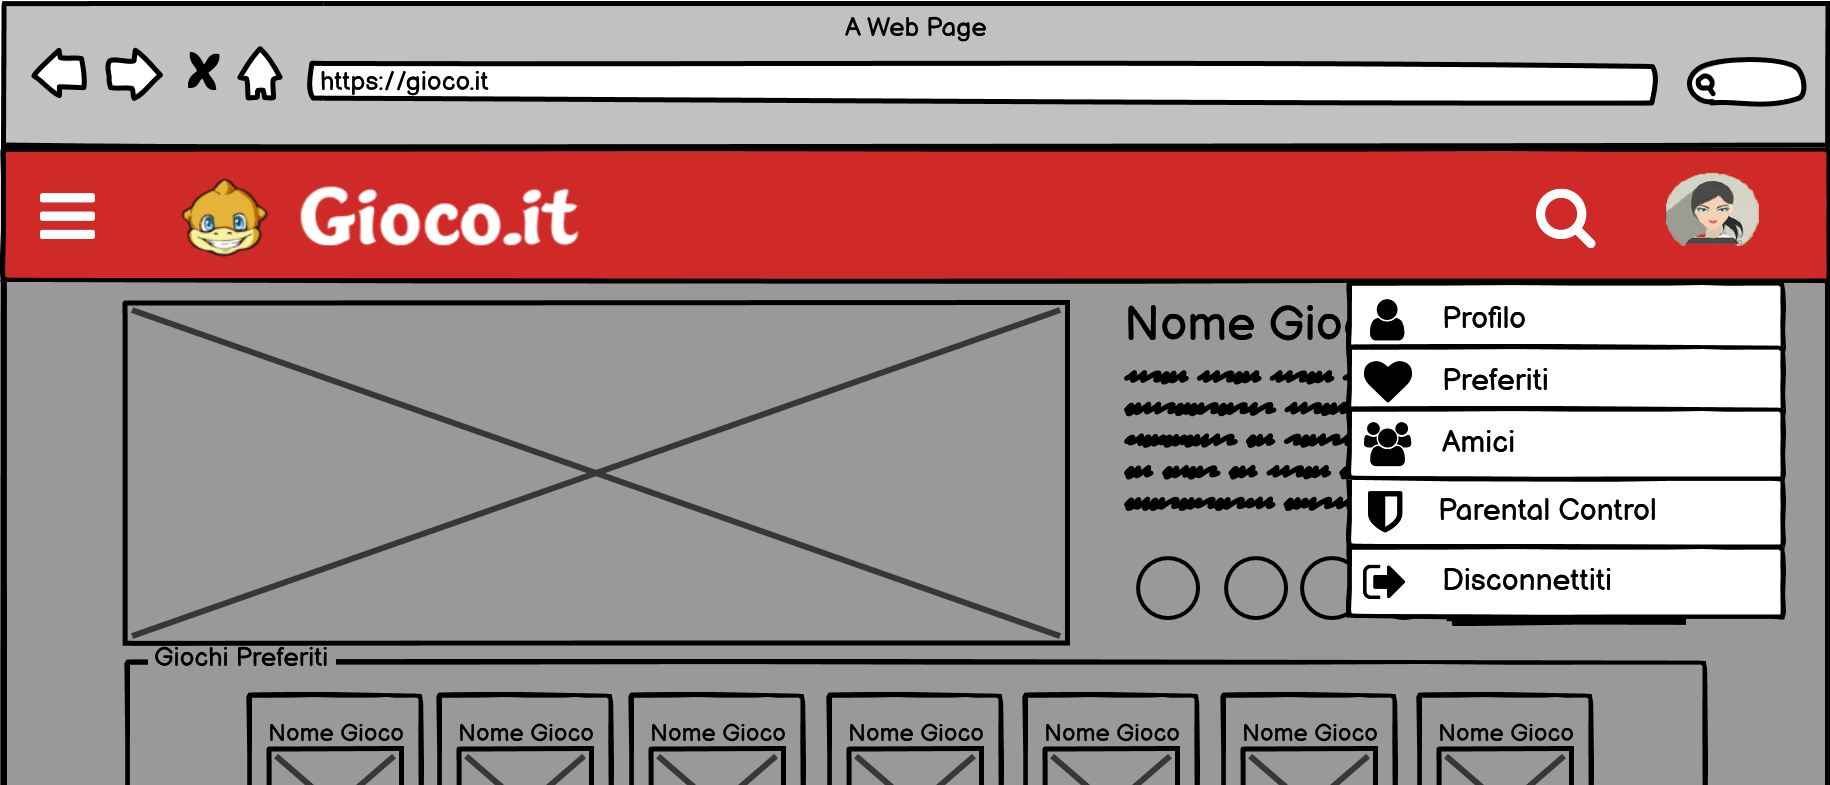
\includegraphics[width=0.9\linewidth]{WProfileMenu (Clear version).png}
        \centering
    \end{figure}

    \begin{figure}[H]
        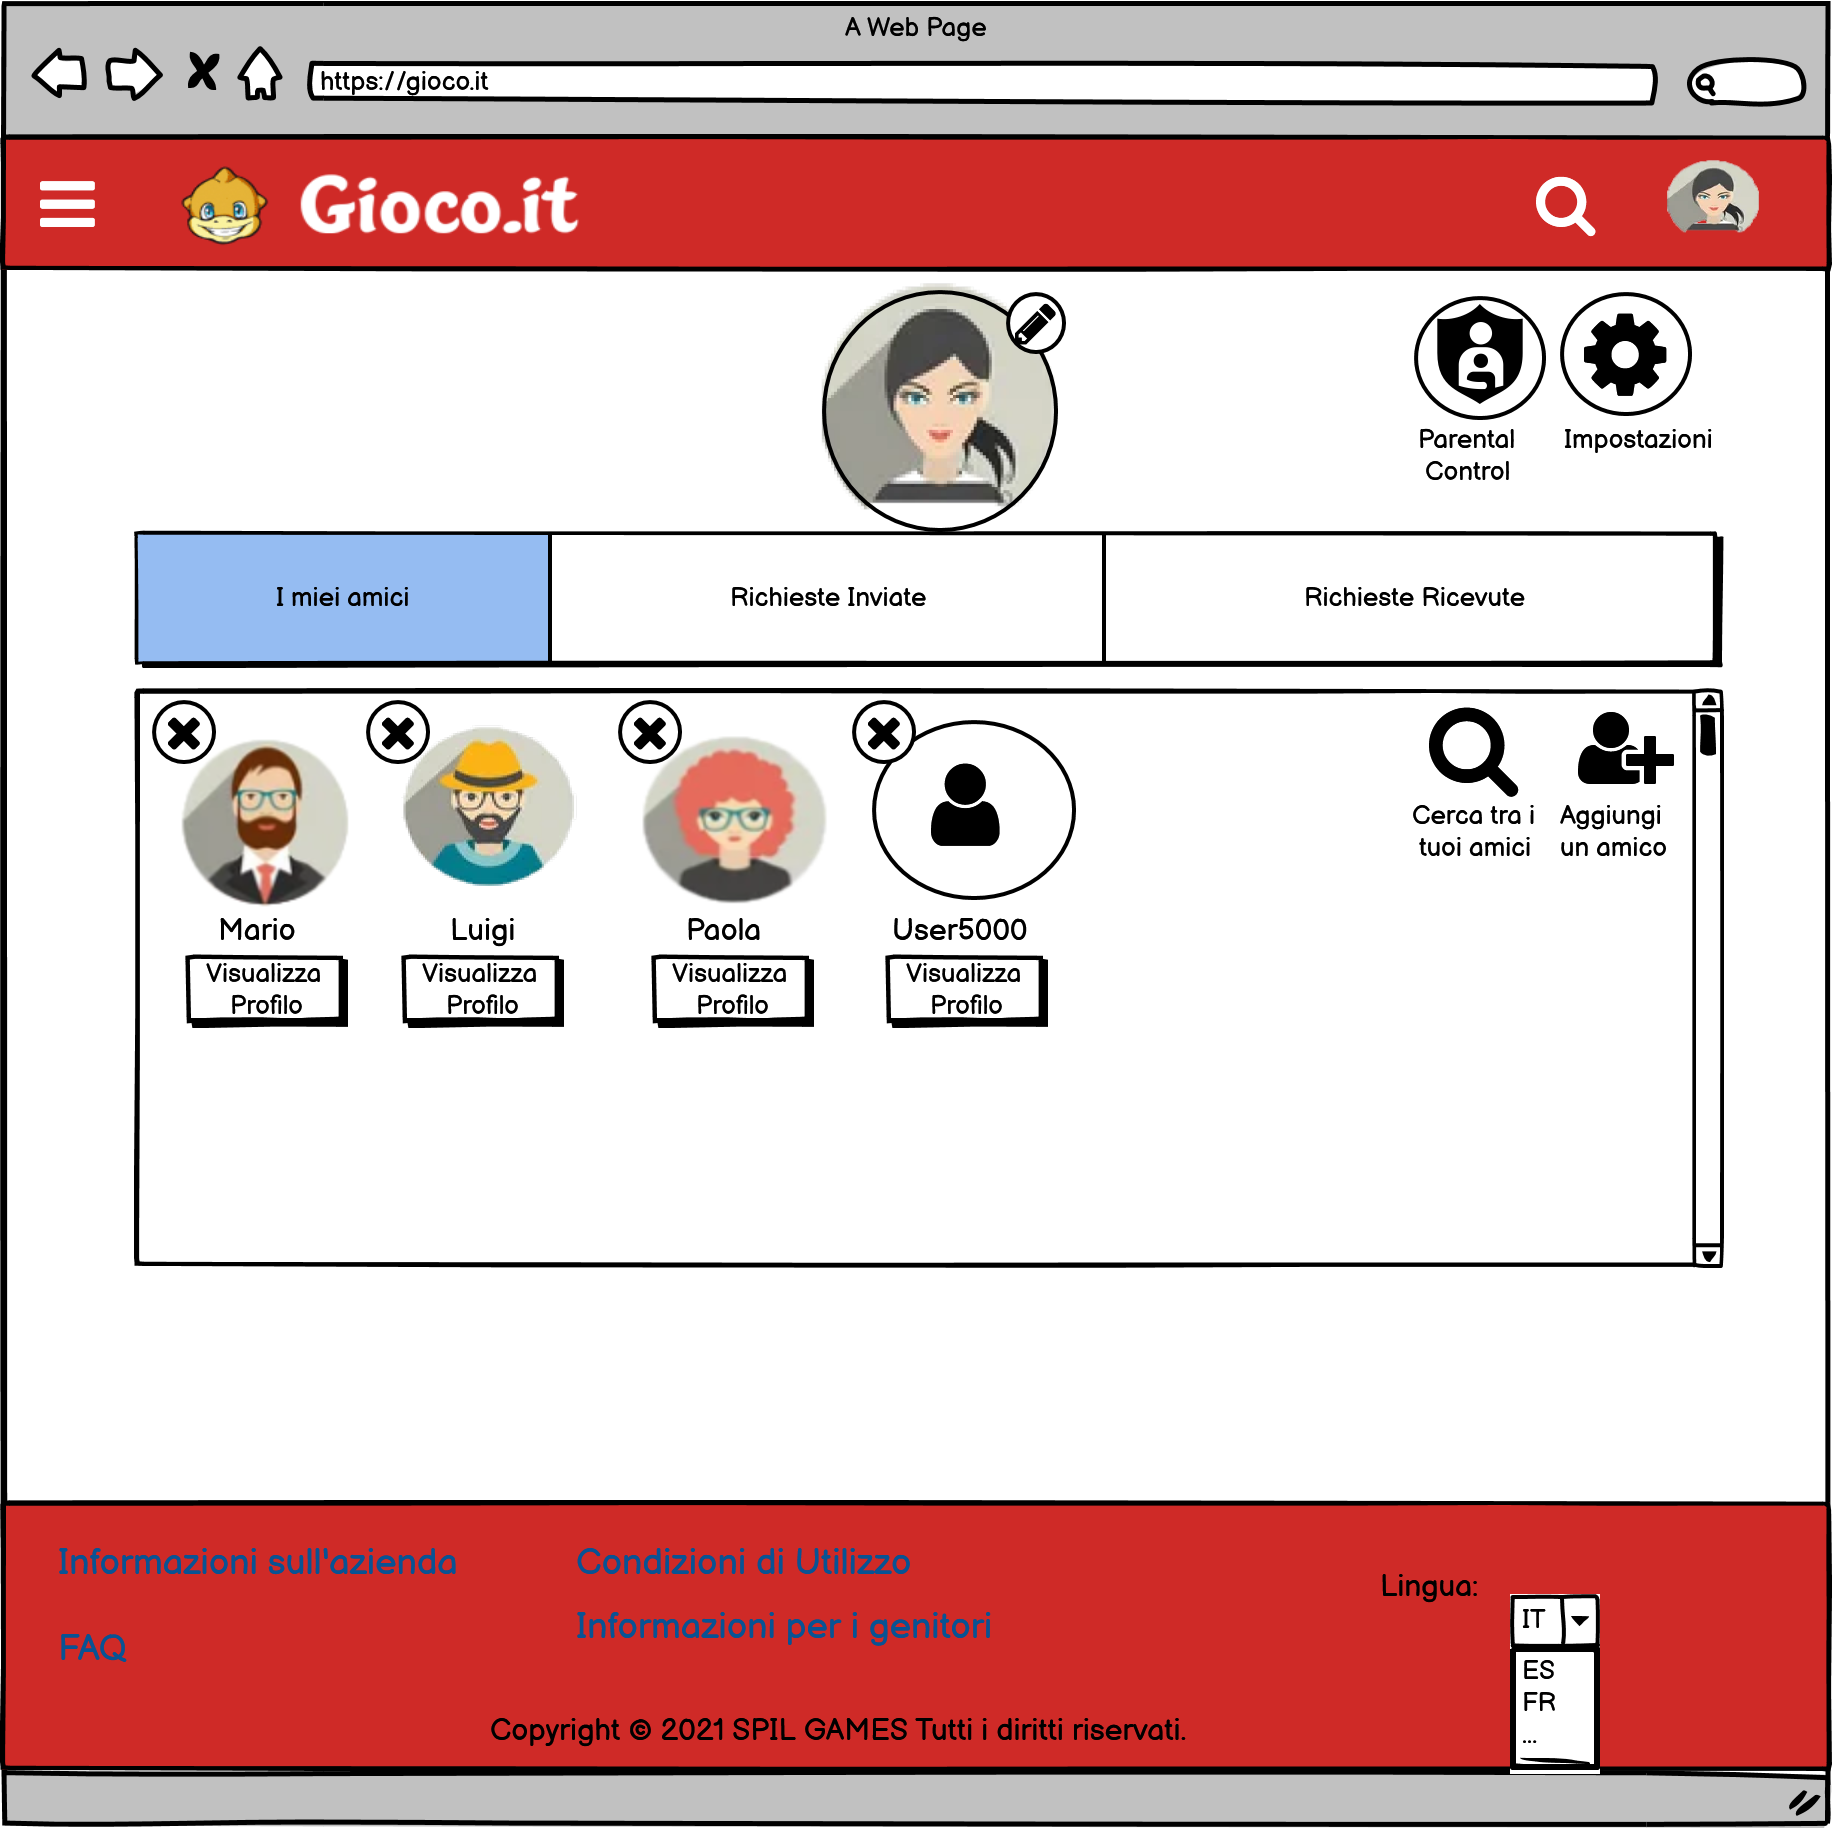
\includegraphics[width=0.9\linewidth]{WAmici1 (Labeled).png}
        \centering
    \end{figure}

    \begin{figure}[H]
        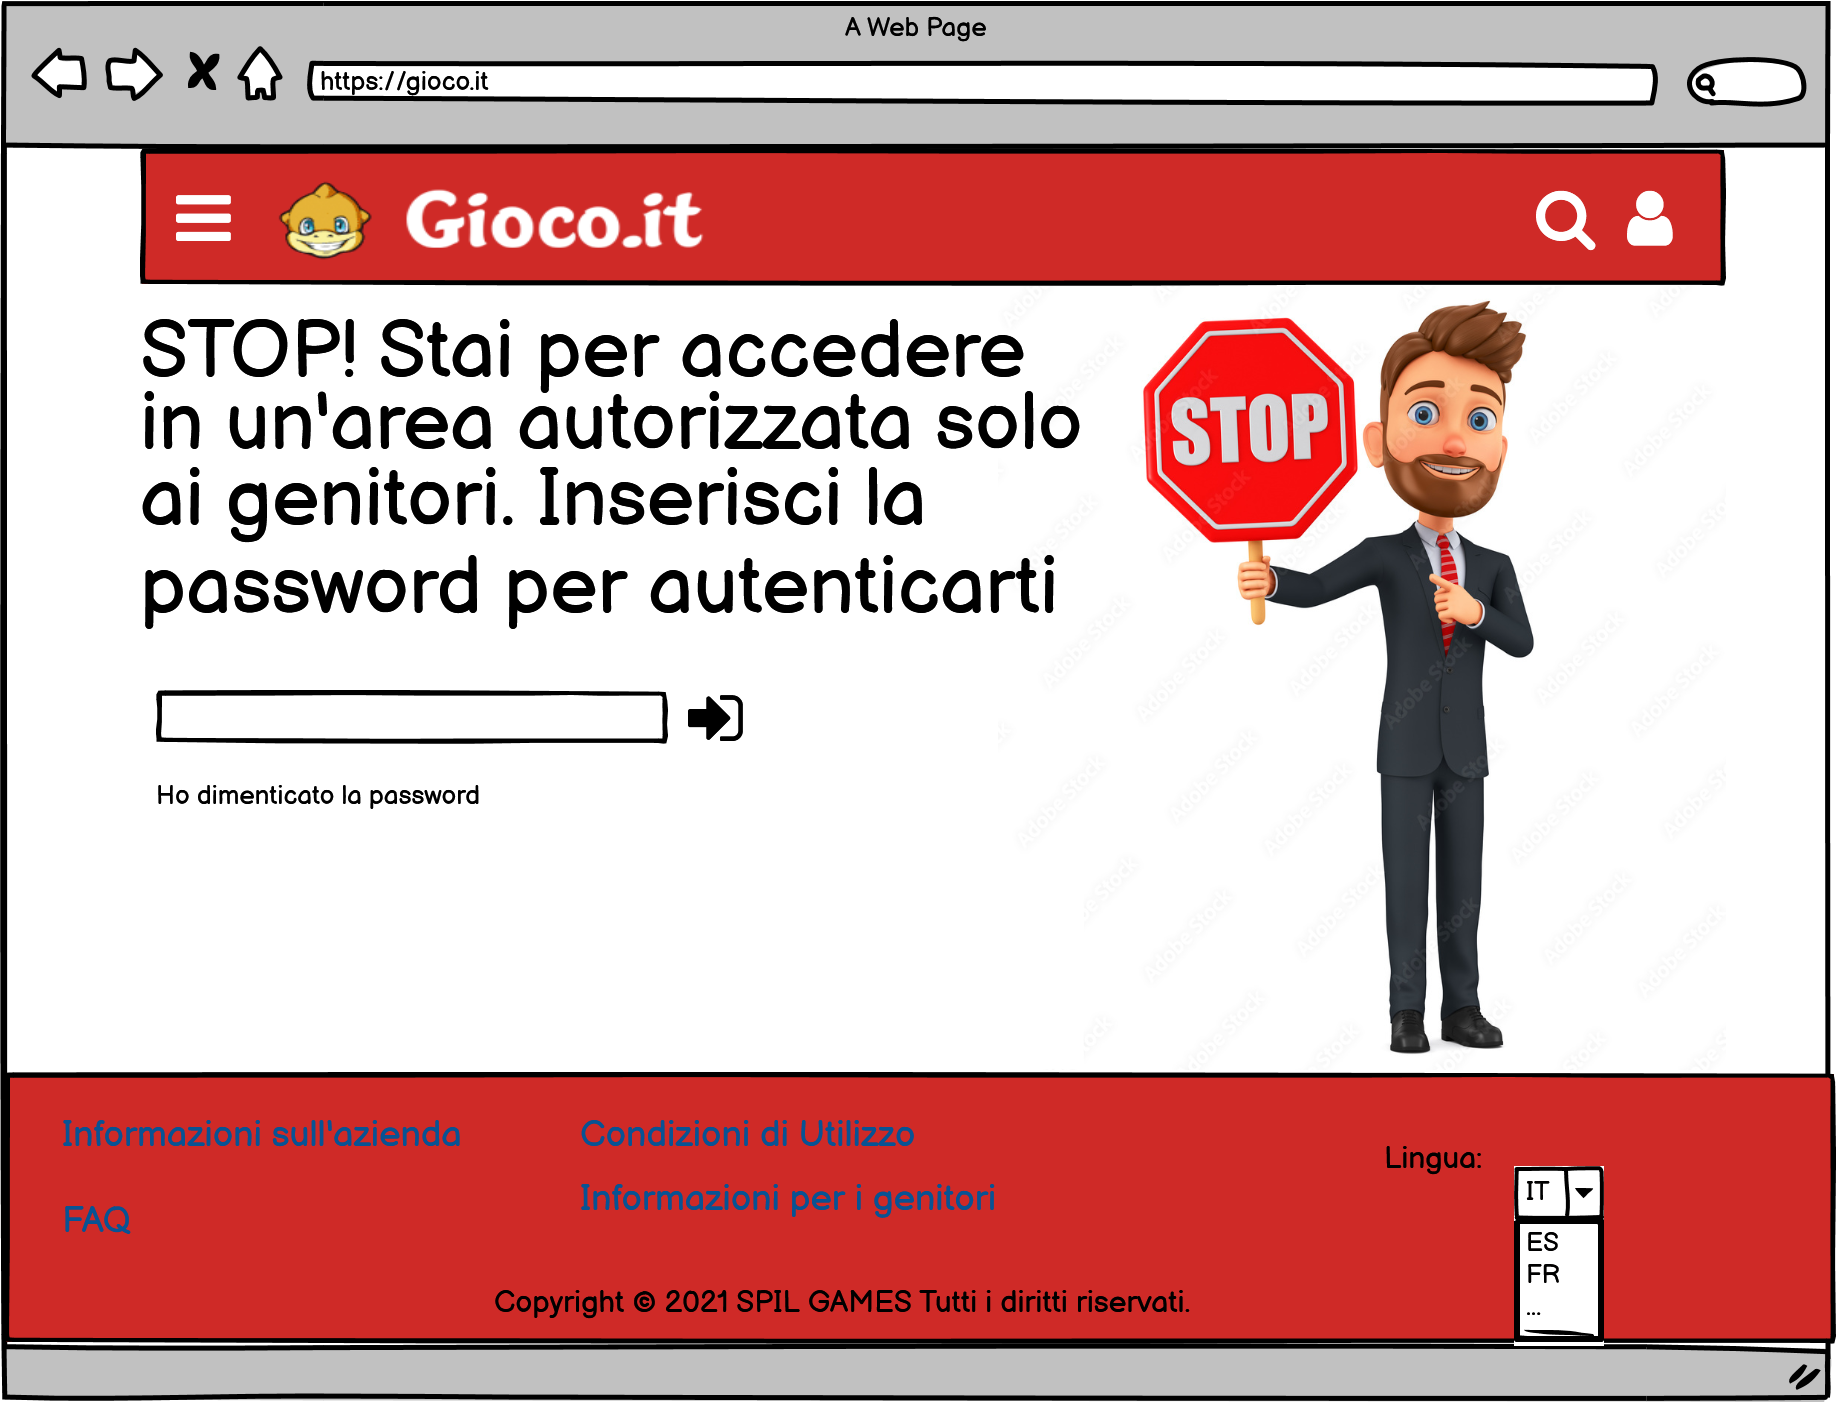
\includegraphics[width=0.9\linewidth]{WParentalControlAcces (Whit Forgotten).png}
        \centering
    \end{figure}

    \begin{figure}[H]
        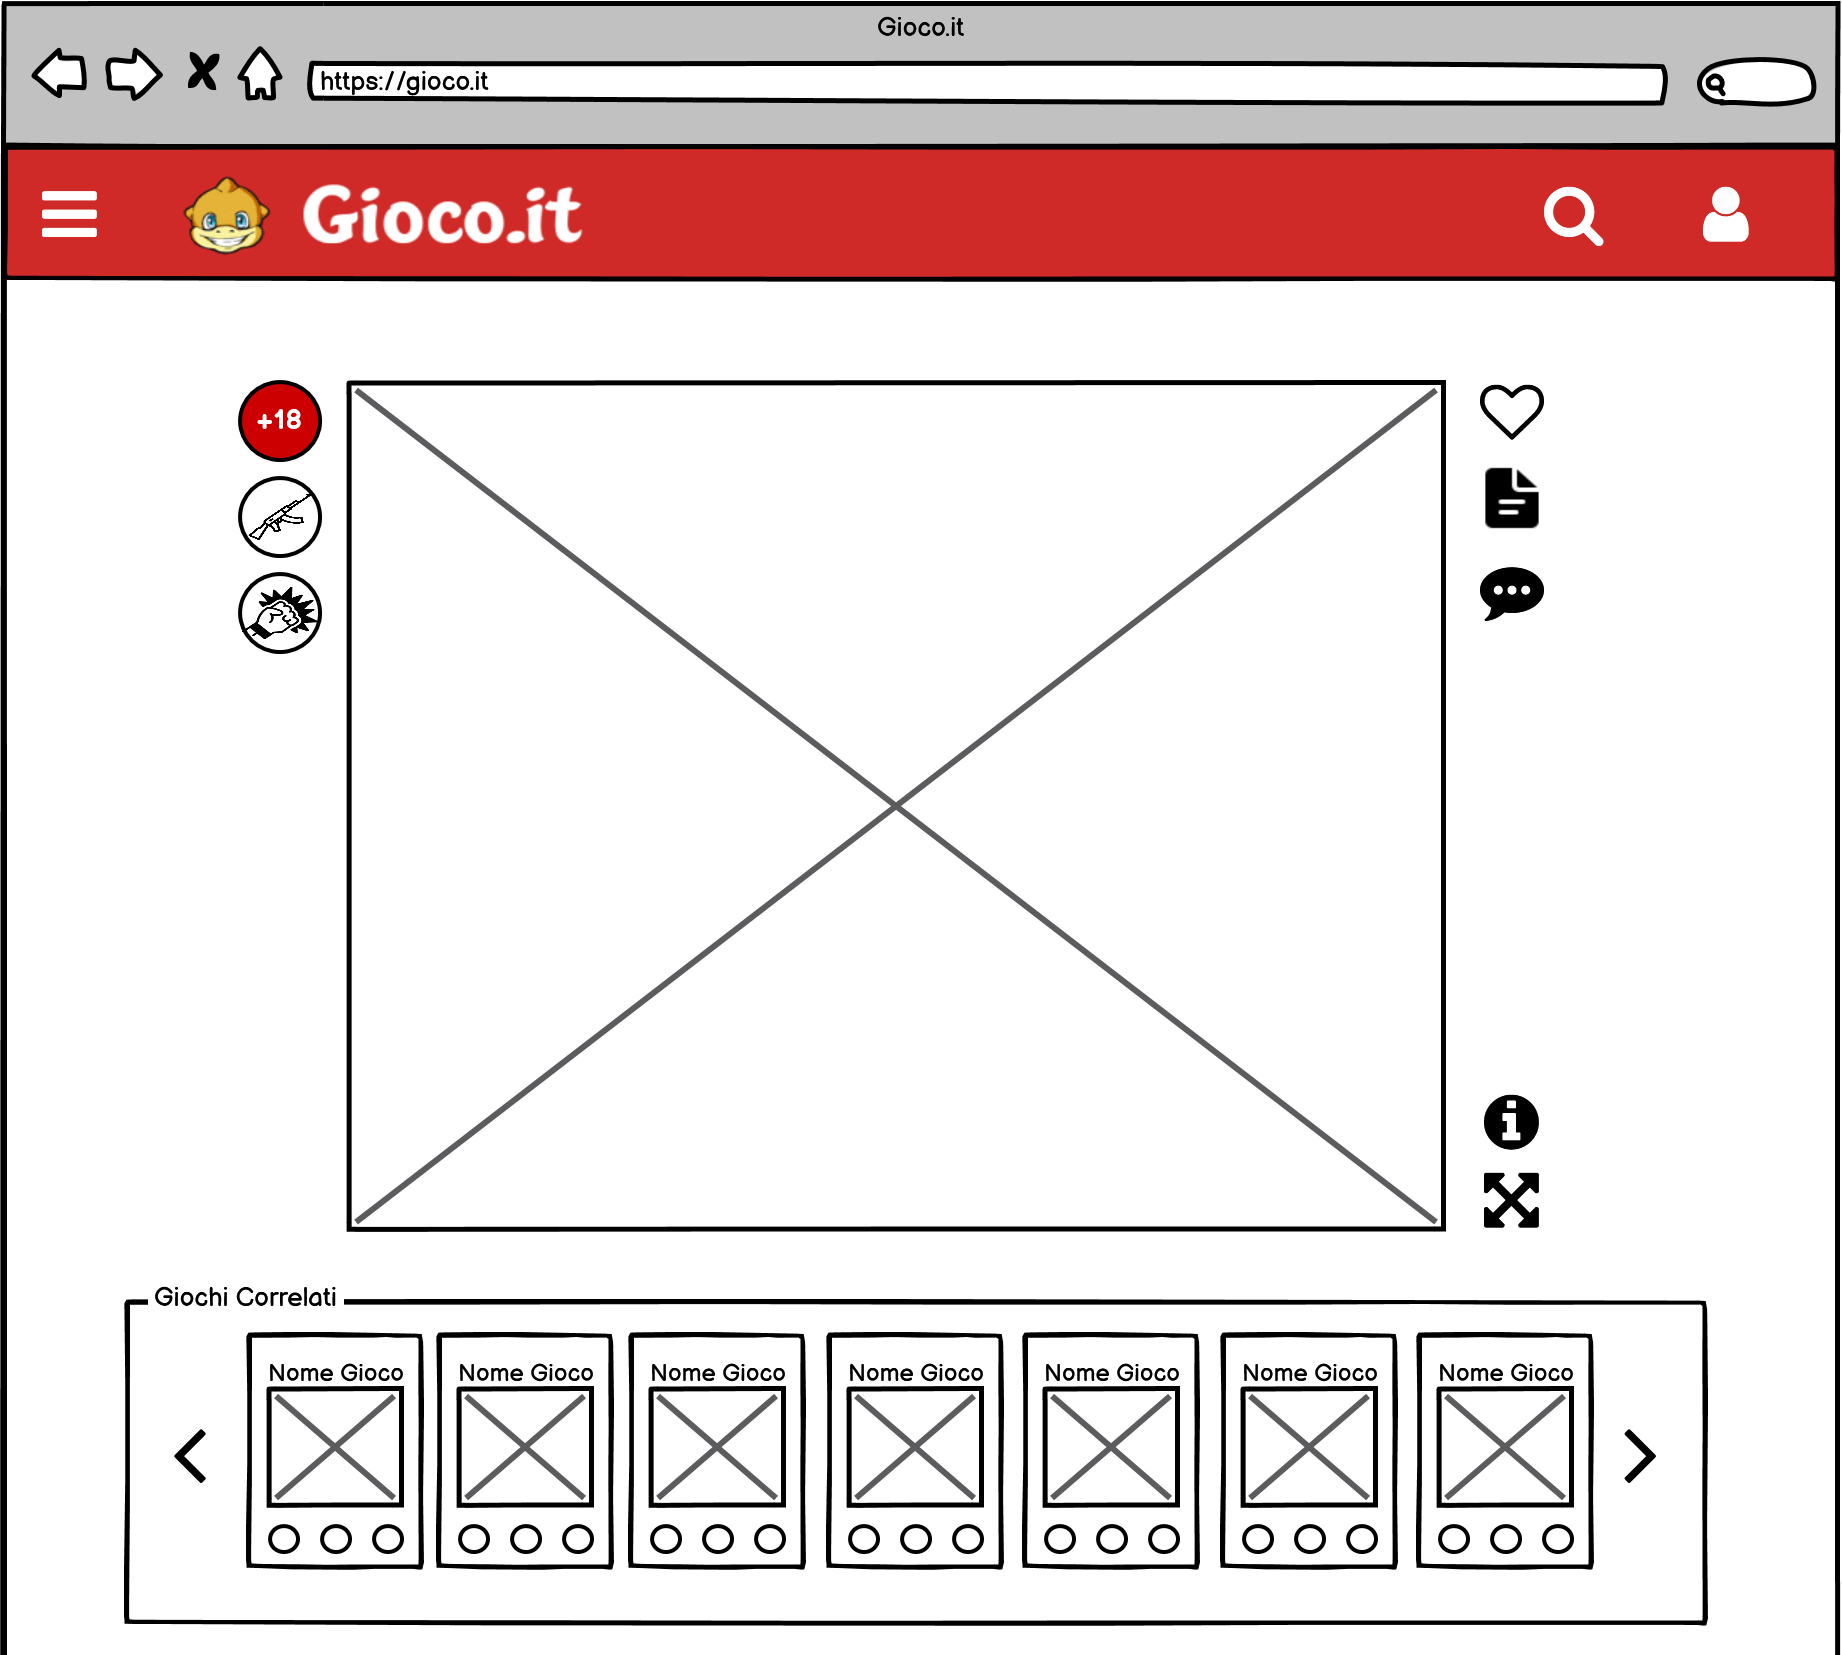
\includegraphics[width=0.9\linewidth]{WGioco_1 (new version).png}
        \centering
    \end{figure}
    
    \chapter{Conclusioni}
    Il nostro lavoro di redesign del sito Gioco.it ha avuto lo scopo di offrire ad un segmento target complementare a quello degli utenti primari (i bambini) una serie di servizi, che possiamo descrivere come fondamentali per l'utilizzo in sicurezza del sistema. Nonostante l'offerta di nuovi servizi si sia rivolta per lo più ad un pubblico adulto abbiamo effettuato un complessivo redesign per rendere il sito più minimale e di facile comprensione, per diminuire al minimo le frizioni che possono esserci tra gli utilizzatori bambini ed il loro scopo: divertirsi ed imparare. \\
    Abbiamo infatti dapprima rivisto la home page, troppo ricca di giochi e disorganizzata, snellendola e preferendo un approccio che accompagna il ragazzo nella scelta del gioco e che offre lui dei nuovi giochi (sezione Gioco del giorno) ma che allo stesso tempo rende semplice ed efficace la ripetizione di task soliti (come l'accesso a giochi preferiti o la scelta dell'ultimo gioco giocato).\\
    Abbiamo poi preso a carico le preoccupazioni dei genitori offrendo loro informazioni utili ai genitori a riguardo dei contenuti del gioco. Se questo non bastasse per farli sentire al sicuro è stata aggiunta la possibilità di impostare un Parental Control, con un'area non accessibile ai ragazzi (accessibile tramite una password diversa) che permette di limitare l'utilizzo del sito ed i suoi contenuti.\\
    Confrontando i risultati dei test SUS tra il testing del sito precedente al nostro design e quelli successivi al nostro design possiamo dire che in media sono aumentati di circa 10 punti.
    Riteniamo che questo nostro design non stravolga il sito, ma sia una sua evoluzione che mantiene i punti di forza e smussa quelli di debolezza, portando il sito al soddisfacimento dei bisogni di un'altra categoria di utenti. Abbiamo, infatti, risolto tutte le problematiche venute fuori dalla preliminare fase di inspezione e testing. 



\end{document}